% =========================================================================
%  LLM-Guided PCA-Latent Corrosion Mask Forecasting — Technical Report
% =========================================================================
\documentclass[11pt,a4paper]{article}

% ── Packages ──────────────────────────────────────────────────────────────
\usepackage[utf8]{inputenc}
\usepackage[T1]{fontenc}
\usepackage{amsmath,amssymb,amsfonts,amsthm}
\usepackage{booktabs}
\usepackage{hyperref}
\usepackage{listings}
\usepackage[margin=2.4cm]{geometry}
\usepackage{graphicx}
\usepackage{xcolor}
\usepackage{enumitem}
\usepackage{algorithm}
\usepackage{algpseudocode}
\usepackage{bm}
\usepackage{mathtools}
\usepackage{microtype}
\usepackage{caption}
\usepackage{subcaption}
\usepackage{tikz}
\usetikzlibrary{arrows.meta,positioning,shapes.geometric,fit}

% ── Colours ───────────────────────────────────────────────────────────────
\definecolor{codegreen}{rgb}{0.0,0.50,0.0}
\definecolor{codegray}{rgb}{0.50,0.50,0.50}
\definecolor{codepurple}{rgb}{0.58,0.0,0.82}
\definecolor{backcolour}{rgb}{0.97,0.97,0.97}
\definecolor{accentblue}{rgb}{0.18,0.31,0.58}

% ── Listing style ─────────────────────────────────────────────────────────
\lstdefinestyle{pythonstyle}{
  backgroundcolor=\color{backcolour},
  commentstyle=\color{codegreen}\itshape,
  keywordstyle=\color{accentblue}\bfseries,
  stringstyle=\color{codepurple},
  basicstyle=\ttfamily\footnotesize,
  breakatwhitespace=false,
  breaklines=true,
  captionpos=b,
  keepspaces=true,
  numbers=left,
  numbersep=6pt,
  numberstyle=\tiny\color{codegray},
  showspaces=false,
  showstringspaces=false,
  showtabs=false,
  tabsize=4,
  frame=single,
  rulecolor=\color{codegray!40},
  language=Python,
  morekeywords={self,True,False,None,as,with,yield,async,await},
}
\lstset{style=pythonstyle}

% ── Hyperref setup ────────────────────────────────────────────────────────
\hypersetup{
  colorlinks=true,
  linkcolor=accentblue,
  citecolor=accentblue,
  urlcolor=accentblue,
}

% ── Math shortcuts ────────────────────────────────────────────────────────
\newcommand{\R}{\mathbb{R}}
\newcommand{\E}{\mathbb{E}}
\newcommand{\1}{\mathds{1}}
\newcommand{\vx}{\mathbf{x}}
\newcommand{\vz}{\mathbf{z}}
\newcommand{\vv}{\mathbf{v}}
\newcommand{\vf}{\mathbf{f}}
\newcommand{\vmu}{\bm{\mu}}
\newcommand{\vdelta}{\bm{\delta}}
\DeclareMathOperator*{\argmin}{arg\,min}
\DeclareMathOperator*{\argmax}{arg\,max}
\DeclareMathOperator{\diag}{diag}

% ── Theorem-like environments ─────────────────────────────────────────────
\theoremstyle{definition}
\newtheorem{definition}{Definition}[section]
\newtheorem{remark}{Remark}[section]

% ══════════════════════════════════════════════════════════════════════════
\title{%
  \textbf{LLM-Guided PCA-Latent Corrosion Mask Forecasting}\\[6pt]
  \Large Technical Report}
\author{Alexander Hermann}
\date{\today}

\graphicspath{{../figures/}}

\begin{document}
\maketitle

% ──────────────────────────────────────────────────────────────────────────
\begin{abstract}
This report documents the mathematical foundations and software architecture
of a corrosion forecasting pipeline designed to predict the temporal evolution
of binary corrosion masks for Mg--4Ag biodegradable alloy wires.  The masks
are derived from in-situ synchrotron nano-CT imaging and captured at ten
discrete degradation time-steps.  The pipeline combines \emph{Principal
Component Analysis} (PCA) via randomised Singular Value Decomposition (SVD),
a \emph{Signed Distance Field} (SDF) representation, $k$-Nearest Neighbour
(kNN) delta prediction in latent space, and a \emph{Large Language Model}
(LLM) that provides a stochastic residual correction to the kNN prior.
Deterministic stabilisers ensure physical plausibility (e.g.\ monotonic
material loss), while Monte Carlo rollouts yield pixel-wise uncertainty
maps.  The entire system is implemented as a modular Python package
(\texttt{corrosion\_forecast}) and evaluated with spatial overlap, boundary
accuracy, and probabilistic calibration metrics.
\end{abstract}

\tableofcontents
\newpage

% ══════════════════════════════════════════════════════════════════════════
%   PART  1 :   MATHEMATICAL  THEORY
% ══════════════════════════════════════════════════════════════════════════
\part{Mathematical Theory}
\label{part:theory}

% ──────────────────────────────────────────────────────────────────────────
\section{Principal Component Analysis via Singular Value Decomposition}
\label{sec:pca}

\subsection{Data Matrix Construction}

Let $T$ denote the total number of temporal snapshots and $S$ the number of
training slice indices.  Each corrosion mask image of resolution $H \times W$
is first converted to a field representation (Section~\ref{sec:sdf}) and then
flattened into a row vector of length $N = H \cdot W$.  Stacking all
$M = S \times T$ training fields yields the data matrix

\begin{equation}
  \mathbf{X} \;=\;
  \begin{pmatrix}
    \vx_1^\top \\ \vx_2^\top \\ \vdots \\ \vx_M^\top
  \end{pmatrix}
  \;\in\; \R^{M \times N}.
  \label{eq:datamatrix}
\end{equation}

\subsection{Mean Subtraction}

The global mean field is
\begin{equation}
  \vmu \;=\; \frac{1}{M}\sum_{i=1}^{M} \vx_i
  \;\in\; \R^{N},
\end{equation}
and the mean-centred data matrix is
\begin{equation}
  \mathbf{X}_c \;=\; \mathbf{X} - \mathbf{1}_M\,\vmu^\top
  \;\in\; \R^{M \times N},
\end{equation}
where $\mathbf{1}_M$ is the $M$-vector of ones.

\subsection{Singular Value Decomposition}

The (economy) SVD of the centred matrix is
\begin{equation}
  \mathbf{X}_c \;=\; \mathbf{U}\,\mathbf{S}\,\mathbf{V}^\top,
  \label{eq:svd}
\end{equation}
where $\mathbf{U}\in\R^{M\times M}$ contains left singular vectors,
$\mathbf{S}=\diag(\sigma_1,\dots,\sigma_{\min(M,N)})$ are singular values
in descending order, and $\mathbf{V}\in\R^{N\times N}$ contains right
singular vectors.  The columns of $\mathbf{V}$ (equivalently the rows of
$\mathbf{V}^\top$) are the \emph{principal component directions}
$\vv_1,\dots,\vv_N$.

\subsection{Truncated Reconstruction}

Retaining only $K \ll \min(M,N)$ components, an arbitrary field $\vx$ is
reconstructed as
\begin{equation}
  \hat{\vx} \;=\; \vmu + \sum_{k=1}^{K} z_k\, \vv_k,
  \label{eq:pca_recon}
\end{equation}
where the \emph{latent coefficients} are
\begin{equation}
  z_k \;=\; (\vx - \vmu)^\top \vv_k, \qquad k=1,\dots,K.
\end{equation}
The latent vector $\vz = (z_1,\dots,z_K)^\top \in \R^K$ provides a
low-dimensional representation of the corrosion field.

\subsection{Explained Variance Ratio}

Each singular value $\sigma_k$ is related to the eigenvalue of the covariance
matrix via $\lambda_k = \sigma_k^2 / (M-1)$.  The fraction of variance
explained by the first $K$ components is
\begin{equation}
  \mathrm{EVR}(K) \;=\;
  \frac{\displaystyle\sum_{k=1}^{K}\lambda_k}
       {\displaystyle\sum_{j=1}^{\min(M,N)}\lambda_j}
  \;=\;
  \frac{\displaystyle\sum_{k=1}^{K}\sigma_k^2}
       {\displaystyle\sum_{j=1}^{\min(M,N)}\sigma_j^2}.
  \label{eq:evr}
\end{equation}

\subsection{Randomised SVD}

For large $M$ and $N$, the full SVD is computationally prohibitive.
Following~\cite{halko2011finding}, we use the \emph{randomised SVD}
algorithm, which approximates the top-$K$ singular triplets in
$\mathcal{O}(MN\log K)$ time rather than $\mathcal{O}(MN\min(M,N))$.  The
algorithm proceeds by:
\begin{enumerate}
  \item Drawing a random Gaussian matrix $\mathbf{\Omega}\in\R^{N\times(K+p)}$,
        where $p$ is a small over-sampling parameter.
  \item Computing the sample matrix $\mathbf{Y}=\mathbf{X}_c\,\mathbf{\Omega}$.
  \item Obtaining an orthonormal basis $\mathbf{Q}$ for the column space of
        $\mathbf{Y}$ via QR decomposition.
  \item Forming the small matrix $\mathbf{B}=\mathbf{Q}^\top\mathbf{X}_c$
        and computing its SVD.
\end{enumerate}
In our implementation, we use \texttt{sklearn.utils.extmath.randomized\_svd}
when available, falling back to \texttt{numpy.linalg.svd} otherwise.

\subsection{Latent Normalisation}

To ensure numerical stability when feeding latent vectors to downstream
predictors, we compute per-component statistics
\begin{equation}
  \bar{z}_k = \frac{1}{M}\sum_{i=1}^{M} z_k^{(i)}, \qquad
  s_k = \sqrt{\frac{1}{M}\sum_{i=1}^{M} \bigl(z_k^{(i)}-\bar{z}_k\bigr)^2 + \epsilon},
\end{equation}
with $\epsilon=10^{-6}$, and work with the normalised latent
$\tilde{z}_k = (z_k - \bar{z}_k)/s_k$ throughout the forecasting pipeline.


% ──────────────────────────────────────────────────────────────────────────
\section{Signed Distance Field (SDF) Representation}
\label{sec:sdf}

\subsection{Definition}

\begin{definition}[Signed Distance Field]
Given a binary material mask $\mathcal{M} \subseteq \R^2$ (the set of
pixels labelled as material), the Signed Distance Field is defined at every
pixel location $\vx$ as
\begin{equation}
  \mathrm{SDF}(\vx) \;=\;
  d_{\mathrm{outside}}(\vx) \;-\; d_{\mathrm{inside}}(\vx),
  \label{eq:sdf_def}
\end{equation}
where
\begin{align}
  d_{\mathrm{inside}}(\vx) &= \inf_{\vy \in \partial\mathcal{M}} \|\vx - \vy\|_2
    \quad\text{for } \vx \in \mathcal{M}, \\
  d_{\mathrm{outside}}(\vx) &= \inf_{\vy \in \partial\mathcal{M}} \|\vx - \vy\|_2
    \quad\text{for } \vx \notin \mathcal{M},
\end{align}
and $\partial\mathcal{M}$ denotes the material boundary.
\end{definition}

By this convention:
\begin{itemize}
  \item $\mathrm{SDF}(\vx) < 0$ for pixels \textbf{inside} the material.
  \item $\mathrm{SDF}(\vx) > 0$ for pixels \textbf{outside} the material.
  \item $\mathrm{SDF}(\vx) = 0$ at the material boundary.
\end{itemize}
In practice, both distance transforms are computed using the Euclidean
Distance Transform (\texttt{scipy.ndimage.distance\_transform\_edt}).

\subsection{Zero Level-Set Recovery}

The material mask can always be recovered from the SDF by thresholding:
\begin{equation}
  \mathcal{M} \;=\; \bigl\{\vx : \mathrm{SDF}(\vx) \le 0\bigr\}.
  \label{eq:sdf_threshold}
\end{equation}

\subsection{Advantages over Raw Binary Masks}

Using SDF representations instead of raw $\{0,255\}$ binary masks for PCA
confers several advantages:

\begin{enumerate}
  \item \textbf{Smoothness:} The SDF is a continuous, piecewise-smooth function.
        Small perturbations of the boundary produce small perturbations of the
        SDF in the $L^2$ norm, whereas binary masks exhibit discontinuous jumps.
  \item \textbf{Boundary sensitivity:} The SDF gradient is largest near the
        boundary (magnitude $=1$ everywhere for exact distance functions),
        ensuring that PCA modes concentrate representational power on the
        shape of the boundary rather than on interior fill.
  \item \textbf{Linear interpolation:} Averaging two SDF fields in PCA latent
        space yields a geometrically meaningful intermediate shape, whereas
        averaging two binary masks produces ambiguous grey values.
  \item \textbf{Reconstruction quality:} Truncated PCA reconstruction of a
        smooth SDF produces a smooth field whose zero level-set gives a clean
        boundary; reconstructing a binary mask introduces ringing artefacts.
\end{enumerate}


% ──────────────────────────────────────────────────────────────────────────
\section{\texorpdfstring{$k$}{k}-Nearest Neighbour Delta Prediction}
\label{sec:knn}

\subsection{Feature Vector Construction}

The kNN predictor operates in the normalised PCA latent space.  At time $t$,
the feature vector for a query is composed of:
\begin{equation}
  \vf \;=\;
  \bigl[\,\tilde{\vz}_{t},\;\; \dot{\tilde{\vz}}_{t},\;\;
         t_{\mathrm{norm}},\;\; \Delta t_{\mathrm{norm}}\,\bigr]
  \;\in\; \R^{2K+2},
  \label{eq:knn_feat}
\end{equation}
where:
\begin{itemize}
  \item $\tilde{\vz}_{t} \in \R^K$ is the normalised latent state at time $t$.
  \item $\dot{\tilde{\vz}}_{t} = \tilde{\vz}_{t} - \tilde{\vz}_{t-1}$ is the
        latent velocity (zero for $t=0$).
  \item $t_{\mathrm{norm}} = t_h / t_{\max}$ and
        $\Delta t_{\mathrm{norm}} = \Delta t_h / t_{\max}$ are the normalised
        current time and step size (in hours), respectively.
\end{itemize}

\subsection{Library Construction}

For each training slice and each pair of consecutive time-steps
$(t,\,t+1)$, we store the pair $(\vf_t,\,\vdelta_t)$ where
$\vdelta_t = \tilde{\vz}_{t+1} - \tilde{\vz}_{t}$ is the ground-truth
latent delta.  The full library is
\begin{equation}
  \mathcal{L} = \bigl\{(\vf^{(i)},\,\vdelta^{(i)})\bigr\}_{i=1}^{|\mathcal{L}|}.
\end{equation}

\subsection{Inverse-Distance Weighted Prediction}

Given a query feature $\vf_q$, we find the $k$ nearest neighbours
$\mathcal{N}_k(\vf_q)$ in $\mathcal{L}$ by Euclidean distance.  For each
neighbour $i \in \mathcal{N}_k$, the distance is
\begin{equation}
  d_i = \|\vf_q - \vf^{(i)}\|_2.
\end{equation}

The inverse-distance weights are
\begin{equation}
  w_i = \frac{1/d_i}{\displaystyle\sum_{j \in \mathcal{N}_k} 1/d_j},
  \qquad i \in \mathcal{N}_k,
  \label{eq:idw}
\end{equation}
with a small additive constant $\epsilon=10^{-6}$ for numerical stability.

The \textbf{weighted mean} (the kNN prior) is
\begin{equation}
  \vdelta_{\mathrm{prior}} = \vmu_{\mathrm{kNN}}
  = \sum_{i \in \mathcal{N}_k} w_i \,\vdelta^{(i)},
  \label{eq:knn_mean}
\end{equation}
and the \textbf{weighted variance} (for uncertainty estimation) is
\begin{equation}
  \sigma_{\mathrm{kNN}}^2
  = \sum_{i \in \mathcal{N}_k} w_i
    \bigl(\vdelta^{(i)} - \vmu_{\mathrm{kNN}}\bigr)^2.
  \label{eq:knn_var}
\end{equation}


% ──────────────────────────────────────────────────────────────────────────
\section{LLM-in-the-Loop Forecasting}
\label{sec:llm}

\subsection{Hybrid Architecture}

The pipeline employs a \emph{hybrid} forecasting strategy: the kNN module
provides a physics-informed, data-driven baseline prediction (the
\emph{prior}), and a Large Language Model (LLM) adds a stochastic
\emph{residual correction} that captures non-linear dependencies beyond
nearest-neighbour interpolation.

The final predicted delta is
\begin{equation}
  \vdelta \;=\;
  \vdelta_{\mathrm{prior}} \;+\; \alpha\,\vdelta_{\mathrm{LLM}},
  \label{eq:delta_hybrid}
\end{equation}
where $\alpha \in [0,1]$ is the \texttt{RESIDUAL\_SCALE} parameter (default
$\alpha = 0.7$) and $\vdelta_{\mathrm{LLM}}$ is the residual vector returned
by the LLM.

\subsection{Prompt Structure}

The LLM receives a single \textbf{JSON payload} as the user message,
containing:
\begin{lstlisting}
{
  "D":            <int: dimension of latent space>,
  "dt_hours":     <float: time-step in hours>,
  "last_latent":  [z_1, z_2, ..., z_K],
  "velocity":     [v_1, v_2, ..., v_K],
  "acceleration": [a_1, a_2, ..., a_K],
  "delta_prior":  [d_1, d_2, ..., d_K],
  "prior_std":    [s_1, s_2, ..., s_K],
  "residual_norm_cap":  <float>,
  "residual_comp_cap":  <float>,
  "rollout_nonce":      <float: for stochastic diversity>,
  "metadata_context":   { ... }
}
\end{lstlisting}

The system prompt instructs the model to return \textbf{only} valid JSON
with a single key \texttt{predicted\_delta} containing exactly $K$ floats.
Explicitly:

\begin{lstlisting}[language={},numbers=none]
Return ONLY JSON. No prose. No markdown.
Output ONLY JSON with exactly one key predicted_delta.
predicted_delta must be a list of exactly D=<K> floats.
Interpret predicted_delta as a RESIDUAL to add to delta_prior.
Keep it small: L2(residual) <= residual_norm_cap
  and abs(component) <= residual_comp_cap.
\end{lstlisting}

\subsection{Kinematic Context}

To help the LLM reason about the dynamics, we provide:
\begin{itemize}
  \item The \textbf{last latent state} $\tilde{\vz}_t$.
  \item The \textbf{velocity} $\dot{\tilde{\vz}}_t = \tilde{\vz}_t - \tilde{\vz}_{t-1}$.
  \item The \textbf{acceleration}
    $\ddot{\tilde{\vz}}_t = \dot{\tilde{\vz}}_t - \dot{\tilde{\vz}}_{t-1}$
    (zero if fewer than three observations are available).
\end{itemize}

\subsection{Rationale for the Hybrid Approach}

\begin{enumerate}
  \item \textbf{kNN provides structure:} The inverse-distance-weighted
        neighbourhood average is fast, purely data-driven, and guaranteed
        to stay within the convex hull of training deltas.  It encodes the
        \emph{typical} magnitude and direction of latent evolution.
  \item \textbf{LLM adds flexibility:} By operating as a residual predictor,
        the LLM need only learn the \emph{correction} to the prior, which
        is typically much smaller than the full delta.  This reduces the
        effective prediction complexity and makes the system more robust
        to LLM hallucinations.
  \item \textbf{Bounded risk:} The residual is capped both in norm and per
        component (see Section~\ref{sec:stabilisers}), so even a poorly
        calibrated LLM output cannot drive the prediction far from the kNN
        baseline.
\end{enumerate}

\subsection{Robust JSON Parsing and Retry Logic}

LLM outputs may deviate from the expected format.  The parsing module
implements a multi-stage recovery strategy:
\begin{enumerate}
  \item \textbf{Strict parsing}: attempt \texttt{json.loads} on the raw response.
  \item \textbf{Regex extraction}: search for an embedded \texttt{\{...\}} JSON blob.
  \item \textbf{Text salvage}: if enabled, extract floating-point numbers from
        potentially truncated text after the key \texttt{predicted\_delta}.
  \item \textbf{Length repair}: trim or zero-pad the vector if its length does
        not match $K$.
  \item \textbf{Conversational retry}: append the malformed response as an
        assistant turn and ask the model to correct itself (up to
        \texttt{LLM\_MAX\_RETRIES} times).
\end{enumerate}


% ──────────────────────────────────────────────────────────────────────────
\section{Deterministic Stabilisers}
\label{sec:stabilisers}

After obtaining the combined delta $\vdelta$ (Equation~\ref{eq:delta_hybrid}),
several deterministic constraints are applied to ensure physical plausibility
and prevent forecast divergence.

\subsection{Training-Derived Caps}
\label{sec:caps}

From all consecutive-step deltas in the training set, we compute:
\begin{itemize}
  \item \textbf{Magnitude cap:} the 95th percentile of $\|\vdelta^{(i)}\|_2$
        across training pairs, scaled by a multiplier $\rho_{\mathrm{mag}}$
        (default 1.2):
        \begin{equation}
          c_{\mathrm{mag}} = \rho_{\mathrm{mag}} \cdot P_{95}\!\bigl(\{\|\vdelta^{(i)}\|_2\}\bigr).
          \label{eq:mag_cap}
        \end{equation}
        If $\|\vdelta\|_2 > c_{\mathrm{mag}}$, the delta is rescaled:
        $\vdelta \leftarrow \vdelta \cdot c_{\mathrm{mag}} / \|\vdelta\|_2$.

  \item \textbf{Per-component cap:} the 99th percentile of
        $|\delta_k^{(i)}|$ for each component $k$, scaled by
        $\rho_{\mathrm{comp}}$ (default 1.2):
        \begin{equation}
          c_k = \rho_{\mathrm{comp}} \cdot P_{99}\!\bigl(\{|\delta_k^{(i)}|\}\bigr).
          \label{eq:comp_cap}
        \end{equation}
        Each component is clipped: $\delta_k \leftarrow \mathrm{clip}(\delta_k,\, -c_k,\, c_k)$.
\end{itemize}

\subsection{Horizon Damping}

For multi-step autoregressive rollouts, prediction uncertainty compounds
with each step.  To counteract drift, the delta magnitude is attenuated
exponentially with the forecast horizon $h$:
\begin{equation}
  \vdelta \;\leftarrow\; \vdelta \cdot \gamma^{\,(h-1)},
  \label{eq:horizon_damp}
\end{equation}
where $\gamma \in (0,1]$ is the damping factor (default $\gamma=0.95$).
The first horizon step ($h=1$) is unmodified.

\subsection{Velocity-Relative Cap}

To prevent the predicted change from being unreasonably large compared to
the observed rate of evolution, we impose
\begin{equation}
  \|\vdelta\|_2 \;\le\; \alpha_v \,\|\dot{\tilde{\vz}}\|_2 + \beta_v,
  \label{eq:vel_cap}
\end{equation}
where $\alpha_v$ (default 6.0) and $\beta_v$ (default 0.2) are tuneable
constants.  If the constraint is violated, $\vdelta$ is rescaled to satisfy
it.  A minimum cap floor of $0.25 \cdot c_{\mathrm{mag}}$ prevents the
constraint from being too restrictive when velocity is very small.

\begin{remark}
When the kNN guide is active, the velocity-relative cap is optionally
disabled (\texttt{DISABLE\_VEL\_CAP\_WHEN\_KNN=True}) because the kNN prior
already implicitly regularises the delta magnitude.
\end{remark}

\subsection{Monotonic SDF Shrinkage}
\label{sec:mono}

Corrosion is an irreversible process: material can only be removed, never
added.  In the SDF representation, material loss corresponds to the SDF
becoming more positive (or less negative).  We enforce this via a
pixel-wise maximum:
\begin{equation}
  \mathrm{SDF}_{t+1}(\vx)
  \;=\; \max\!\bigl(\mathrm{SDF}_{\mathrm{pred}}(\vx),\;
                     \mathrm{SDF}_{t}(\vx)\bigr)
  \quad \forall\, \vx.
  \label{eq:mono_sdf}
\end{equation}
Since $\mathrm{SDF}(\vx) \le 0$ indicates material and the maximum operator
only \emph{increases} SDF values, this guarantees
$\mathcal{M}_{t+1} \subseteq \mathcal{M}_t$ (monotonic shrinkage).

\subsection{Optional SDF Smoothing}

Before thresholding, the predicted SDF may be lightly smoothed with a
Gaussian filter ($\sigma=0.8$~px) to suppress high-frequency artefacts
introduced by PCA truncation:
\begin{equation}
  \mathrm{SDF}_{\mathrm{smooth}} = G_\sigma * \mathrm{SDF}_{\mathrm{pred}},
\end{equation}
where $G_\sigma$ is the Gaussian kernel.

\subsection{Mask Post-Processing}

After thresholding the SDF to obtain a binary mask, morphological
post-processing is applied in the following order:
\begin{enumerate}
  \item \textbf{Fill holes:} close interior voids using
        \texttt{binary\_fill\_holes}.
  \item \textbf{Remove small components:} discard connected components
        with fewer than 200 pixels.
  \item \textbf{Largest component:} keep only the largest connected
        component (the alloy wire cross-section).
  \item \textbf{Monotonic mask shrinkage:} intersect the predicted mask with the
        previous-step mask: $\mathcal{M}_{t+1} \leftarrow \mathcal{M}_{t+1} \cap \mathcal{M}_t$.
\end{enumerate}


% ──────────────────────────────────────────────────────────────────────────
\section{Monte Carlo Uncertainty Quantification}
\label{sec:mc}

\subsection{Stochastic Rollouts}

With the LLM temperature $\tau > 0$, each call to the language model
produces a different residual correction, inducing stochasticity in the
forecast.  We perform $R$ independent autoregressive rollouts (default
$R=8$), each seeded with a distinct \texttt{rollout\_nonce}.  The LLM
effective temperature decays across horizons:
\begin{equation}
  \tau_{\mathrm{eff}}(h) = \tau_0 \cdot \eta^{\max(0,\,h-1)},
\end{equation}
where $\eta$ (default 0.98) is the horizon temperature decay.

\subsection{Probability Map}

The pixel-wise probability of material survival is estimated from the
ensemble of rollout predictions:
\begin{equation}
  P(\text{material}\,|\,\vx)
  \;=\; \frac{1}{R}\sum_{r=1}^{R}
        \mathbb{I}\!\bigl[\vx \in \mathcal{M}^{(r)}\bigr],
  \label{eq:prob_map}
\end{equation}
where $\mathcal{M}^{(r)}$ is the predicted material mask from rollout $r$
and $\mathbb{I}[\cdot]$ is the indicator function.

\subsection{Mean Prediction}

The consensus (mean) prediction thresholds the probability map at 0.5:
\begin{equation}
  \hat{\mathcal{M}} = \bigl\{\vx : P(\text{material}\,|\,\vx) \ge 0.5\bigr\}.
  \label{eq:mean_pred}
\end{equation}

\begin{remark}
Regions where $P(\text{material}\,|\,\vx)$ is close to 0.5 indicate high
uncertainty.  These typically localise along the advancing corrosion front,
providing physically meaningful uncertainty estimates.
\end{remark}


% ──────────────────────────────────────────────────────────────────────────
\section{Evaluation Metrics}
\label{sec:metrics}

\subsection{Spatial Overlap Metrics}

Let $A$ and $B$ denote the ground-truth and predicted material masks,
respectively.

\subsubsection{Intersection over Union (IoU)}
\begin{equation}
  \mathrm{IoU}(A,B) = \frac{|A \cap B|}{|A \cup B|},
  \label{eq:iou}
\end{equation}
where $|\cdot|$ denotes the pixel count.

\subsubsection{S{\o}rensen--Dice Coefficient}
\begin{equation}
  \mathrm{Dice}(A,B) = \frac{2\,|A \cap B|}{|A| + |B|}.
  \label{eq:dice}
\end{equation}

\begin{remark}
IoU and Dice are related by $\mathrm{Dice} = 2\,\mathrm{IoU}/(1+\mathrm{IoU})$,
so Dice is always $\ge$ IoU for the same prediction.  IoU is the stricter
metric.
\end{remark}

\subsection{Boundary F1-Score (BF1)}
\label{sec:bf1}

The boundary F1-score evaluates boundary localisation accuracy.  First,
extract boundary pixels of each mask via morphological erosion:
\begin{equation}
  \partial A = A \;\oplus\; \bigl(A \ominus \mathcal{B}\bigr),
\end{equation}
where $\ominus$ is erosion and $\oplus$ is symmetric difference (XOR).
With a tolerance of $\tau$ pixels (implemented as dilation by $\tau$ iterations):
\begin{align}
  \mathrm{Prec}_\tau &= \frac{|\partial B \cap D_\tau(\partial A)|}{|\partial B|}, \\[4pt]
  \mathrm{Rec}_\tau  &= \frac{|\partial A \cap D_\tau(\partial B)|}{|\partial A|},
\end{align}
where $D_\tau(\cdot)$ denotes dilation by $\tau$ pixels.  The Boundary
F1-score is
\begin{equation}
  \mathrm{BF1}_\tau = \frac{2\,\mathrm{Prec}_\tau\,\mathrm{Rec}_\tau}
                           {\mathrm{Prec}_\tau + \mathrm{Rec}_\tau}.
  \label{eq:bf1}
\end{equation}

\subsection{Probabilistic Calibration Metrics}

Let $p_i \in [0,1]$ be the predicted probability that pixel $i$ is material,
and $y_i \in \{0,1\}$ the ground-truth label.

\subsubsection{Brier Score}
\begin{equation}
  \mathrm{BS} = \frac{1}{N}\sum_{i=1}^{N}(p_i - y_i)^2.
  \label{eq:brier}
\end{equation}
Lower is better; a perfect deterministic predictor achieves $\mathrm{BS}=0$.

\subsubsection{Negative Log-Likelihood (NLL)}
\begin{equation}
  \mathrm{NLL} = -\frac{1}{N}\sum_{i=1}^{N}
    \bigl[y_i\log(p_i+\epsilon) + (1-y_i)\log(1-p_i+\epsilon)\bigr],
  \label{eq:nll}
\end{equation}
with $\epsilon = 10^{-6}$ for numerical stability.

\subsubsection{Expected Calibration Error (ECE)}

Partition pixels into $B$ bins by predicted probability.  Let $\mathcal{B}_b$
be the set of pixels in bin $b$, with $n_b = |\mathcal{B}_b|$, mean
confidence $\bar{p}_b$, and empirical accuracy $\bar{y}_b$.  Then:
\begin{equation}
  \mathrm{ECE} = \sum_{b=1}^{B} \frac{n_b}{N}
    \bigl|\bar{y}_b - \bar{p}_b\bigr|.
  \label{eq:ece}
\end{equation}
ECE is visualised using a \emph{reliability diagram} (Section~\ref{sec:plotting}).


% ──────────────────────────────────────────────────────────────────────────
\section{Auto-Tune PCA}
\label{sec:autotune}

\subsection{Motivation}

The number of principal components $K$ and the training set size jointly
determine reconstruction fidelity.  Too few components lose fine-grained
boundary detail; too many overfit noise and inflate the latent dimension
for downstream predictors.

\subsection{Grid Search Protocol}

The auto-tune procedure performs a grid search over
$(\texttt{n\_train}, K)$ using \emph{oracle reconstruction} on a held-out
validation set.  Oracle reconstruction projects the ground-truth field
onto the PCA basis with $K$ components and then thresholds to obtain
a material mask:
\begin{equation}
  \hat{\vx}^{(K)} = \vmu + \sum_{k=1}^{K}
    \bigl[(\vx - \vmu)^\top \vv_k\bigr]\,\vv_k,
  \qquad
  \hat{\mathcal{M}}^{(K)} = \bigl\{\vx : \hat{\vx}^{(K)}(\vx) \le 0\bigr\}.
\end{equation}

To reduce computational cost, all fields are spatially downsampled by a
factor of 2 (default), and only a subset of time-steps
$\{0, 3, 6, 9\}$ is used.

\subsection{Quality Thresholds}

The smallest $K$ satisfying \emph{all} of the following is selected as
$K_{\mathrm{LLM}}$:
\begin{align}
  \overline{\mathrm{IoU}}(K)  &\ge 0.985, \label{eq:tune_iou}\\
  \overline{\mathrm{Dice}}(K) &\ge 0.990, \label{eq:tune_dice}\\
  \overline{\mathrm{BF1}}(K)  &\ge 0.930. \label{eq:tune_bf1}
\end{align}

The reconstruction dimensionality $K_{\mathrm{recon}} \ge K_{\mathrm{LLM}}$
is selected as the point of diminishing returns, where the marginal IoU
and Dice gain from an additional component drops below $5\times 10^{-4}$.

\subsection{Subspace Stability}
\label{sec:stability}

To verify that the PCA basis is robust to training set composition, we
fit two bases on independent random subsets and measure the
\emph{principal angles} between the resulting $K$-dimensional subspaces:
\begin{equation}
  \theta_j = \arccos\bigl(\sigma_j(\mathbf{V}_A^{(K)\top}\mathbf{V}_B^{(K)})\bigr),
  \quad j = 1,\dots,K,
\end{equation}
where $\sigma_j(\cdot)$ are singular values.  A candidate is accepted only
if $\bar{\theta} \le 8^\circ$ (mean principal angle).


% ══════════════════════════════════════════════════════════════════════════
%   PART  2 :   CODE  ARCHITECTURE  AND  DOCUMENTATION
% ══════════════════════════════════════════════════════════════════════════
\part{Code Architecture and Documentation}
\label{part:code}

% ──────────────────────────────────────────────────────────────────────────
\section{Package Structure}
\label{sec:structure}

The pipeline is implemented as a single Python package with the following
layout:

\begin{lstlisting}[language={},numbers=none,frame=single,
  basicstyle=\ttfamily\small]
corrosion_forecast/
|-- __init__.py
|-- config.py
|-- data_loading.py
|-- sdf_utils.py
|-- pca.py
|-- metrics.py
|-- knn.py
|-- llm_interface.py
|-- forecasting.py
|-- autotune.py
|-- ablation.py
|-- plotting.py
|-- main.py
`-- requirements.txt
\end{lstlisting}

Dependencies:

\begin{lstlisting}[language={},numbers=none,frame=single,
  basicstyle=\ttfamily\small]
numpy>=1.24      scipy>=1.10     matplotlib>=3.7
pandas>=2.0      imageio>=2.31   requests>=2.28
scikit-learn>=1.3
\end{lstlisting}


% ──────────────────────────────────────────────────────────────────────────
\section{Module Descriptions}
\label{sec:modules}

%--------------------------------------------------------------------------
\subsection{\texttt{config.py} --- Global Configuration}
\label{sec:mod_config}

\textbf{Purpose:} Centralises all tuneable hyperparameters, file-system
paths, and feature flags so that experiments are reproducible and
modifications require editing only a single file.

\subsubsection{Key Constants}

\begin{table}[h]
\centering\small
\begin{tabular}{lll}
\toprule
\textbf{Group} & \textbf{Parameter} & \textbf{Default} \\
\midrule
Paths     & \texttt{BASE\_DIR}           & \texttt{../Corrosion\_Masks} (or \texttt{\$CORROSION\_BASE\_DIR}) \\
          & \texttt{METADATA\_CSV}       & \texttt{<BASE\_DIR>/metadata.csv} \\
          & \texttt{NUM\_TIMESTEPS}      & 10 \\
\midrule
LLM       & \texttt{OPENROUTER\_API\_KEY}& \texttt{\$OPENROUTER\_API\_KEY} \\
          & \texttt{LLM\_MODEL}          & \texttt{openai/gpt-4o-mini} \\
          & \texttt{LLM\_TEMPERATURE}    & 0.6 \\
          & \texttt{LLM\_MAX\_TOKENS}    & 600 \\
          & \texttt{LLM\_MAX\_RETRIES}   & 2 \\
\midrule
PCA       & \texttt{K\_LLM}              & 40 \\
          & \texttt{K\_PCS\_MAX}         & 80 \\
          & \texttt{NUM\_TRAIN\_SLICES}  & 400 \\
\midrule
kNN       & \texttt{KNN\_K}              & 16 \\
          & \texttt{KNN\_MAX\_SLICES}    & 300 \\
          & \texttt{RESIDUAL\_SCALE}     & 0.7 \\
\midrule
Stabilisers & \texttt{HORIZON\_DAMP}     & 0.95 \\
            & \texttt{VEL\_REL\_MULT}    & 6.0 \\
            & \texttt{VEL\_REL\_BIAS}    & 0.20 \\
\midrule
Experiment  & \texttt{NUM\_TEST\_SLICES} & 2 \\
            & \texttt{TEST\_START\_TIMES}& $[3, 5]$ \\
            & \texttt{NUM\_ROLLOUTS}     & 8 \\
\bottomrule
\end{tabular}
\caption{Selected configuration parameters and their defaults.}
\label{tab:config}
\end{table}

\subsubsection{Dependencies}
Standard library only (\texttt{os}), plus \texttt{numpy} for dtype
constants.

%--------------------------------------------------------------------------
\subsection{\texttt{data\_loading.py} --- Dataset I/O}
\label{sec:mod_data}

\textbf{Purpose:} Handles all file-system interaction: reading TIFF
corrosion mask slices, parsing the metadata CSV, binarisation, and
in-memory frame caching.

\subsubsection{Key Functions}

\begin{lstlisting}
def load_frame_uint8(
    slice_idx: int, t: int, use_cache: bool = True
) -> Optional[np.ndarray]:
    """Load a single grayscale frame as uint8.
    Returns None if the file does not exist."""

def load_slice_across_time(
    slice_idx: int, use_cache: bool = False
) -> Optional[List[np.ndarray]]:
    """Load one slice index across all NUM_TIMESTEPS time-steps.
    Returns list of (H, W) uint8 images, or None if any missing."""

def get_total_slice_count() -> int:
    """Count .tif files in the first time-step folder."""

def load_times_from_metadata() -> np.ndarray:
    """Return degradation times (hours) from metadata.csv."""

def binarize_0_255(img: np.ndarray, thr: int = 128) -> np.ndarray:
    """Threshold to {0, 255}."""

def to_material_bool(img_0_255: np.ndarray) -> np.ndarray:
    """Convert {0,255} mask to boolean (True = material)."""

def from_material_bool(material_bool: np.ndarray) -> np.ndarray:
    """Inverse of to_material_bool."""

def measure_area_material(material_bool: np.ndarray) -> int:
    """Count material pixels."""
\end{lstlisting}

\subsubsection{Frame Caching}

A module-level dictionary \texttt{\_FRAME\_CACHE} maps
\texttt{(slice\_idx, t)} to the loaded \texttt{uint8} array.  The
cache is transparent to callers and can be cleared via
\texttt{clear\_frame\_cache()}.

\subsubsection{Data Convention}

In the TIFF files, pixel value~0 (black) denotes \textbf{material}
and pixel value~255 (white) denotes \textbf{background/void}.  The
helper \texttt{to\_material\_bool} implements \texttt{img == 0}.

\subsubsection{Dependencies}
\texttt{imageio}, \texttt{numpy}, \texttt{pandas}, \texttt{config}.

%--------------------------------------------------------------------------
\subsection{\texttt{sdf\_utils.py} --- SDF Utilities}
\label{sec:mod_sdf}

\textbf{Purpose:} Converts between boolean material masks and Signed
Distance Fields, and provides morphological post-processing routines.

\subsubsection{Key Functions}

\begin{lstlisting}
def material_to_sdf(material_bool: np.ndarray) -> np.ndarray:
    """Boolean mask -> SDF (float32). Negative inside material."""

def sdf_to_material(sdf: np.ndarray) -> np.ndarray:
    """SDF -> boolean mask via zero level-set (SDF <= 0)."""

def keep_largest_component(mask_bool: np.ndarray) -> np.ndarray:
    """Keep only the largest connected component."""

def remove_small_components(
    mask_bool: np.ndarray, min_pixels: int = 200
) -> np.ndarray:
    """Remove components smaller than min_pixels."""

def postprocess_material(
    pred_material: np.ndarray,
    prev_material: np.ndarray = None,
) -> np.ndarray:
    """Apply cascade: fill holes -> remove small ->
    keep largest -> monotonic shrink."""

def smooth_sdf(sdf: np.ndarray) -> np.ndarray:
    """Optional Gaussian smoothing (sigma from config)."""
\end{lstlisting}

\subsubsection{Post-Processing Cascade}

The \texttt{postprocess\_material} function applies, in order:
\begin{enumerate}
  \item \texttt{binary\_fill\_holes} (if \texttt{FILL\_HOLES}).
  \item \texttt{remove\_small\_components} (if \texttt{MIN\_COMPONENT\_PIXELS} $> 0$).
  \item \texttt{keep\_largest\_component} (if \texttt{ENFORCE\_SINGLE\_COMPONENT}).
  \item Monotonic shrinkage via boolean AND with \texttt{prev\_material}
        (if \texttt{ENFORCE\_MONOTONIC\_SHRINK}).
\end{enumerate}
Each step is gated by the corresponding configuration flag.

\subsubsection{Dependencies}
\texttt{scipy.ndimage}, \texttt{numpy}, \texttt{config}.

%--------------------------------------------------------------------------
\subsection{\texttt{pca.py} --- PCA Basis Fitting}
\label{sec:mod_pca}

\textbf{Purpose:} Fits a global PCA basis from training slices via
(randomised) SVD, and provides projection/reconstruction utilities.

\subsubsection{Key Functions}

\begin{lstlisting}
def fit_global_pca(
    num_slices: int,
    max_index: int,
    k_max: int = 60,
    seed: int = 0,
) -> Tuple[np.ndarray, np.ndarray, np.ndarray, np.ndarray]:
    """Fit PCA basis from training slices.
    Returns: (mean_field, Vt, z_mean, z_std)."""

def project_field(
    field_2d: np.ndarray, mean_field: np.ndarray, Vt: np.ndarray
) -> np.ndarray:
    """Project a 2D field onto PCA basis -> latent z."""

def reconstruct_field(
    z: np.ndarray, mean_field: np.ndarray,
    Vt: np.ndarray, H: int, W: int
) -> np.ndarray:
    """Reconstruct a 2D field from latent vector z."""
\end{lstlisting}

\subsubsection{Implementation Details}

\begin{itemize}
  \item Training slice IDs are randomly sampled up to \texttt{num\_slices}
        from IDs in $[0, \texttt{max\_index})$.
  \item For each slice, \emph{all} $T$ time-steps are included in the
        training matrix, yielding up to $T \times \texttt{num\_slices}$ rows.
  \item If \texttt{scikit-learn} is available, \texttt{randomized\_svd} is
        used; otherwise the code falls back to full SVD.
  \item The function returns both the PCA basis (\texttt{mean\_field}, \texttt{Vt})
        and the latent normalisation statistics (\texttt{z\_mean}, \texttt{z\_std}).
\end{itemize}

\subsubsection{Dependencies}
\texttt{numpy}, \texttt{sklearn} (optional), \texttt{data\_loading},
\texttt{sdf\_utils}, \texttt{config}.

%--------------------------------------------------------------------------
\subsection{\texttt{metrics.py} --- Evaluation Metrics}
\label{sec:mod_metrics}

\textbf{Purpose:} Implements all evaluation metrics used for mask
quality assessment and probabilistic calibration.

\subsubsection{Key Functions}

\begin{lstlisting}
def iou(gt: np.ndarray, pr: np.ndarray) -> float:
    """Intersection over Union for boolean masks."""

def dice(gt: np.ndarray, pr: np.ndarray) -> float:
    """Sorensen-Dice coefficient for boolean masks."""

def boundary_f1(
    gt: np.ndarray, pr: np.ndarray, tol: int = 1
) -> float:
    """Boundary F1-score with tolerance (dilation)."""

def brier_score(probs: np.ndarray, y: np.ndarray) -> float:
    """Mean squared error between probabilities and labels."""

def binary_nll(
    probs: np.ndarray, y: np.ndarray, eps: float = 1e-6
) -> float:
    """Negative log-likelihood for binary predictions."""

def expected_calibration_error(
    probs: np.ndarray, y: np.ndarray, n_bins: int = 15
) -> float:
    """Expected Calibration Error (ECE)."""
\end{lstlisting}

\subsubsection{Dependencies}
\texttt{numpy}, \texttt{scipy.ndimage} (for boundary extraction in BF1).

%--------------------------------------------------------------------------
\subsection{\texttt{knn.py} --- kNN Delta Predictor}
\label{sec:mod_knn}

\textbf{Purpose:} Constructs a reference library of (feature, delta) pairs
from training sequences and provides inverse-distance-weighted $k$-nearest
neighbour predictions in PCA latent space.

\subsubsection{Key Functions}

\begin{lstlisting}
def build_knn_library(
    train_ids: list,
    mean_field: np.ndarray,
    Vt: np.ndarray,
    z_mean: np.ndarray,
    z_std: np.ndarray,
    k_llm: int,
    times_h_all: np.ndarray,
    max_slices: int = 300,
    seed: int = 0,
) -> Dict[str, np.ndarray]:
    """Build kNN library. Returns dict with keys
    'X' (features), 'Y' (deltas), 'tmax'."""

def knn_predict_delta(
    knn_lib: Dict[str, np.ndarray],
    z_last: np.ndarray,
    vel: np.ndarray,
    t_hours: float,
    dt_hours: float,
    k: int = 16,
) -> Tuple[np.ndarray, np.ndarray]:
    """Predict next-step delta via IDW kNN.
    Returns (mean_delta, std_delta)."""
\end{lstlisting}

\subsubsection{Feature Construction}

The internal function \texttt{\_feat\_from\_state} builds the feature vector
as defined in Equation~\eqref{eq:knn_feat}: the last $K$-dimensional
normalised latent, the velocity vector, and two normalised time scalars.
This yields a feature of dimension $2K+2$.

\subsubsection{Dependencies}
\texttt{numpy}, \texttt{data\_loading}, \texttt{pca}, \texttt{config}.

%--------------------------------------------------------------------------
\subsection{\texttt{llm\_interface.py} --- LLM API Interface}
\label{sec:mod_llm}

\textbf{Purpose:} Handles prompt construction, HTTP communication with
the OpenRouter API, and robust JSON parsing of LLM responses.

\subsubsection{Key Functions}

\begin{lstlisting}
def build_llm_prompt(
    latents_norm_hist_top: np.ndarray,
    dt_h: float,
    rollout_nonce: Optional[float] = None,
    meta_row: Optional[Dict] = None,
    delta_prior: Optional[np.ndarray] = None,
    prior_std: Optional[np.ndarray] = None,
    residual_norm_cap: Optional[float] = None,
    residual_comp_cap: Optional[float] = None,
) -> str:
    """Construct the user-message prompt as JSON payload."""

def parse_llm_delta(
    text: str,
    D: int,
    allow_length_repair: bool = False,
    allow_text_salvage: bool = False,
) -> Tuple[Optional[np.ndarray], Dict]:
    """Parse LLM response -> delta vector of length D.
    Multi-stage: strict JSON, regex, salvage, length repair."""

def call_llm_delta(
    latents_norm_hist_top: np.ndarray,
    dt_h: float,
    rollout_nonce: Optional[float] = None,
    meta_row: Optional[Dict] = None,
    horizon: int = 1,
    delta_prior: Optional[np.ndarray] = None,
    prior_std: Optional[np.ndarray] = None,
    residual_norm_cap: Optional[float] = None,
    residual_comp_cap: Optional[float] = None,
) -> Tuple[np.ndarray, str, int, Dict]:
    """Full LLM call with retries.
    Returns (delta_vec, raw_text, http_status, info)."""
\end{lstlisting}

\subsubsection{Retry and Recovery Strategy}

The call loop (up to \texttt{LLM\_MAX\_RETRIES}$+1$ attempts) follows
Algorithm~\ref{alg:llm_retry}.

\begin{algorithm}[h]
\caption{LLM call with progressive recovery}
\label{alg:llm_retry}
\begin{algorithmic}[1]
\For{attempt $= 0, 1, \dots, \texttt{MAX\_RETRIES}$}
  \State Send prompt to LLM via HTTP POST
  \State Parse response with strict JSON
  \If{parse succeeds and length matches $K$}
    \State \Return parsed delta
  \EndIf
  \If{length mismatch and retries remain}
    \State Append repair message; \textbf{continue}
  \EndIf
  \If{parse failure and retries remain}
    \State Append correction message; \textbf{continue}
  \EndIf
  \State Attempt text salvage and length repair (last resort)
  \If{salvage succeeds} \Return salvaged delta \EndIf
  \State \textbf{raise} RuntimeError
\EndFor
\end{algorithmic}
\end{algorithm}

\subsubsection{HTTP Details}

\begin{itemize}
  \item Endpoint: \texttt{https://openrouter.ai/api/v1/chat/completions}.
  \item Authentication: Bearer token via \texttt{OPENROUTER\_API\_KEY}.
  \item The \texttt{response\_format} is set to \texttt{\{"type":"json\_object"\}}
        when \texttt{USE\_RESPONSE\_FORMAT\_JSON=True}, requesting structured output.
  \item The effective temperature decays with horizon:
        $\tau_{\mathrm{eff}} = \tau_0 \cdot 0.98^{h-1}$.
\end{itemize}

\subsubsection{Dependencies}
\texttt{json}, \texttt{re}, \texttt{requests}, \texttt{numpy}, \texttt{config}.

%--------------------------------------------------------------------------
\subsection{\texttt{forecasting.py} --- SDF Forecasting Engine}
\label{sec:mod_forecasting}

\textbf{Purpose:} Implements the single-step SDF forecast
(kNN prior $+$ LLM residual $+$ stabilisers) and the Monte Carlo
rollout loop for multi-step autoregressive prediction.

\subsubsection{Key Functions}

\begin{lstlisting}
def compute_training_caps(
    train_ids: List[int],
    mean_field: np.ndarray,
    Vt: np.ndarray,
    z_mean: np.ndarray,
    z_std: np.ndarray,
    k_llm: int,
    max_slices: int = 250,
    seed: int = 0,
) -> Dict[str, np.ndarray]:
    """Compute magnitude and per-component caps from
    training GT deltas."""

def clip_delta_to_training(
    delta: np.ndarray,
    caps: Optional[Dict],
    horizon: int = 1,
) -> np.ndarray:
    """Apply training caps + horizon damping."""

def apply_velocity_relative_cap(
    delta: np.ndarray,
    vel: np.ndarray,
    mult: float = 6.0,
    bias: float = 0.2,
    min_cap: Optional[float] = None,
) -> np.ndarray:
    """Cap delta magnitude relative to velocity."""

def forecast_next_sdf(
    history_sdfs: List[np.ndarray],
    history_times_h: np.ndarray,
    mean_field: np.ndarray,
    Vt: np.ndarray,
    z_mean: np.ndarray,
    z_std: np.ndarray,
    k_llm: int,
    meta_df=None,
    horizon: int = 1,
    rollout_nonce: Optional[float] = None,
    caps: Optional[Dict] = None,
    knn_lib: Optional[Dict] = None,
) -> Tuple[np.ndarray, Dict]:
    """Single-step SDF forecast. Returns (sdf_next, debug_dict)."""

def rollout_mc(
    full_gt_imgs: List[np.ndarray],
    times_h_all: np.ndarray,
    start_t: int,
    mean_field: np.ndarray,
    Vt: np.ndarray,
    z_mean: np.ndarray,
    z_std: np.ndarray,
    k_llm: int,
    caps: Optional[Dict] = None,
    meta_df=None,
    knn_lib: Optional[Dict] = None,
    n_rollouts: int = 8,
    verbose: bool = True,
) -> Tuple[List[Dict], List[np.ndarray]]:
    """Run R autoregressive rollouts from start_t.
    Returns (records, final_preds)."""
\end{lstlisting}

\subsubsection{Single-Step Pipeline (\texttt{forecast\_next\_sdf})}

The function implements the complete single-step pipeline:
\begin{enumerate}
  \item Project history SDFs into normalised PCA latent space.
  \item Compute kNN prior delta $\vdelta_{\mathrm{prior}}$ and uncertainty $\sigma$.
  \item Compute residual caps: $\|\vdelta_{\mathrm{LLM}}\|_2 \le
        \texttt{RESIDUAL\_NORM\_FRAC} \cdot c_{\mathrm{mag}}$ and per-component cap
        $\max(0.25,\; 3\cdot\mathrm{median}(\sigma))$.
  \item Call LLM for residual correction.
  \item Combine: $\vdelta = \vdelta_{\mathrm{prior}} + \alpha\cdot\vdelta_{\mathrm{LLM}}$.
  \item Apply training caps (Section~\ref{sec:caps}).
  \item Apply velocity-relative cap (Equation~\ref{eq:vel_cap}).
  \item Update latent: $\tilde{\vz}_{t+1} = \tilde{\vz}_t + \vdelta$.
  \item Reconstruct SDF from updated physical-space latent.
  \item Smooth SDF, enforce monotonic shrinkage (Section~\ref{sec:mono}).
\end{enumerate}

\subsubsection{Dependencies}
\texttt{numpy}, \texttt{data\_loading}, \texttt{knn},
\texttt{llm\_interface}, \texttt{metrics}, \texttt{pca},
\texttt{sdf\_utils}, \texttt{config}.

%--------------------------------------------------------------------------
\subsection{\texttt{autotune.py} --- PCA Auto-Tuning}
\label{sec:mod_autotune}

\textbf{Purpose:} Performs a downsampled grid search over PCA
hyperparameters $(n_{\mathrm{train}}, K)$ to automatically select values
that meet quality thresholds while ensuring subspace stability.

\subsubsection{Key Functions}

\begin{lstlisting}
def preload_autotune_fields(
    slice_ids: List[int],
    timesteps: List[int],
    downsample_factor: int = 2,
) -> None:
    """Eagerly load fields into cache for fast grid search."""

def fit_pca_on_indices(
    indices: List[int],
    k_fit_max: int,
    timesteps: List[int],
    downsample_factor: int = 2,
    seed: int = 0,
    use_cache: bool = True,
) -> Tuple[np.ndarray, np.ndarray, Tuple[int, int]]:
    """Fit PCA basis on downsampled fields."""

def oracle_score_curve(
    val_indices: List[int],
    mean_field: np.ndarray,
    Vt: np.ndarray,
    K_grid: List[int],
    timesteps: List[int],
    downsample_factor: int = 2,
    use_cache: bool = True,
) -> pd.DataFrame:
    """Evaluate oracle reconstruction for each K.
    Returns DataFrame with columns K, iou_mean, dice_mean, bf1_mean."""

def subspace_distance_deg(
    VtA: np.ndarray, VtB: np.ndarray, K: int
) -> Tuple[float, float]:
    """Mean and max principal angle (degrees) between
    two K-dim subspaces."""

def auto_tune_pca(
    train_max_index: int, seed: int = 0
) -> Tuple[int, int, int]:
    """Grid-search for (n_train, K_LLM, K_PCS_MAX).
    Returns (tuned_n_train, tuned_k_llm, tuned_k_recon)."""
\end{lstlisting}

\subsubsection{Grid Configuration}

The search grid is defined in \texttt{config.py}:
\begin{itemize}
  \item \texttt{TUNE\_TRAIN\_GRID}: $[400, 800]$ training slices.
  \item \texttt{TUNE\_K\_GRID}: $[40, 60, 80, 120, 160]$ components.
  \item \texttt{TUNE\_TIMESTEPS}: $[0, 3, 6, 9]$ sampled time-steps.
  \item \texttt{TUNE\_DOWNSAMPLE}: factor 2 spatial downsampling.
  \item \texttt{TUNE\_VAL\_SLICES}: 25 held-out validation slices.
\end{itemize}

\subsubsection{Selection Logic}

\begin{enumerate}
  \item For each $n_{\mathrm{train}}$, fit PCA on downsampled training fields.
  \item Evaluate oracle reconstruction on validation set for each $K$.
  \item Select smallest $K_{\mathrm{LLM}}$ meeting IoU/Dice/BF1 thresholds.
  \item Select $K_{\mathrm{recon}}$ at diminishing-returns elbow.
  \item Verify subspace stability via principal angles (Section~\ref{sec:stability}).
  \item Among all stable candidates, select the one with the smallest
        $n_{\mathrm{train}}$ and then the smallest $K_{\mathrm{LLM}}$.
\end{enumerate}

\subsubsection{Dependencies}
\texttt{numpy}, \texttt{pandas}, \texttt{sklearn} (optional),
\texttt{data\_loading}, \texttt{metrics}, \texttt{pca}, \texttt{sdf\_utils},
\texttt{config}.

%--------------------------------------------------------------------------
\subsection{\texttt{ablation.py} --- Ablation Study Runner}
\label{sec:mod_ablation}

\textbf{Purpose:} Compares pipeline variants by temporarily overriding
configuration parameters and running the evaluation loop.  Supports
checkpoint/resume via \texttt{pickle} serialisation.

\subsubsection{Key Functions}

\begin{lstlisting}
def run_ablation_variant(
    name: str,
    valid_slices: List[int],
    times_h_all: np.ndarray,
    mean_field: np.ndarray,
    Vt: np.ndarray,
    z_mean: np.ndarray,
    z_std: np.ndarray,
    k_llm: int,
    caps: Optional[Dict],
    meta_df,
    knn_lib: Optional[Dict],
    n_rollouts: int,
    llm_temperature: Optional[float] = None,
    residual_scale: Optional[float] = None,
    use_knn_guide: Optional[bool] = None,
) -> Tuple[List[Dict], float]:
    """Run one ablation variant. Returns (rows, runtime_s)."""

def run_all_ablations(
    valid_slices: List[int],
    times_h_all: np.ndarray,
    mean_field: np.ndarray,
    Vt: np.ndarray,
    z_mean: np.ndarray,
    z_std: np.ndarray,
    k_llm: int,
    caps: Optional[Dict],
    meta_df,
    knn_lib: Optional[Dict],
) -> pd.DataFrame:
    """Run all four ablation variants with checkpoint/resume."""
\end{lstlisting}

\subsubsection{Ablation Variants}

\begin{table}[h]
\centering\small
\begin{tabular}{lcccc}
\toprule
\textbf{Variant} & \textbf{Rollouts} & \textbf{Temperature} &
  \textbf{Residual scale} & \textbf{kNN} \\
\midrule
MC ensemble (baseline)   & $R=8$  & 0.60 & 0.70 & yes \\
Single-shot              & 1      & 0.60 & 0.70 & yes \\
Deterministic            & 1      & 0.00 & 0.70 & yes \\
kNN-only (no LLM)        & 1      & 0.60 & 0.00 & yes \\
\bottomrule
\end{tabular}
\caption{Ablation study variants.}
\label{tab:ablation}
\end{table}

\subsubsection{Checkpoint/Resume}

After each variant completes, the accumulated rows are serialised to
\texttt{ablation\_partial.pkl}.  On restart, completed variants (identified
by name) are skipped.  This ensures that long-running ablation studies
survive interruptions.

\subsubsection{Dependencies}
\texttt{pandas}, \texttt{numpy}, \texttt{requests}, \texttt{data\_loading},
\texttt{forecasting}, \texttt{config}.

%--------------------------------------------------------------------------
\subsection{\texttt{plotting.py} --- Visualisation Routines}
\label{sec:mod_plotting}
\label{sec:plotting}

\textbf{Purpose:} Provides 11 publication-ready visualisation functions
using only \texttt{matplotlib} (no \texttt{seaborn} dependency).  All
functions apply a consistent style via \texttt{rcParams}.

\subsubsection{Available Plots}

\begin{enumerate}
  \item \textbf{\texttt{plot\_mask\_timeseries}} --- Raw mask sequence across
        all time-steps for a single slice.
  \item \textbf{\texttt{plot\_area\_vs\_time}} --- Material pixel count
        versus degradation time.
  \item \textbf{\texttt{plot\_explained\_variance}} --- Cumulative PCA
        explained variance versus $K$.
  \item \textbf{\texttt{plot\_pca\_reconstructions}} --- Side-by-side ground
        truth versus PCA reconstructions at various $K$ values.
  \item \textbf{\texttt{plot\_eigenimages}} --- First $n$ principal component
        images (``corrosion modes'').
  \item \textbf{\texttt{plot\_metric\_vs\_horizon}} --- Mean $\pm$ std of a
        metric (IoU, Dice, area error) versus forecast horizon.
  \item \textbf{\texttt{plot\_ablation\_comparison}} --- Multi-variant
        comparison (mean $\pm$ std) on the same axes.
  \item \textbf{\texttt{plot\_delta\_over\_baseline}} --- $\Delta$IoU gain of
        each variant over the kNN-only baseline.
  \item \textbf{\texttt{plot\_gallery}} --- Side-by-side GT, mean prediction,
        XOR difference, and $P(\text{material})$ uncertainty map.
  \item \textbf{\texttt{plot\_reliability\_diagram}} --- Calibration curve
        with ECE annotation.
  \item \textbf{\texttt{plot\_risk\_coverage}} --- Risk (mean pixel error)
        versus coverage for uncertainty utility assessment.
\end{enumerate}

\subsubsection{Dependencies}
\texttt{matplotlib}, \texttt{numpy}, \texttt{pandas}.

%--------------------------------------------------------------------------
\subsection{\texttt{main.py} --- Pipeline Orchestrator}
\label{sec:mod_main}

\textbf{Purpose:} Serves as the single entry point that orchestrates the
entire pipeline from data loading to final plots.

\subsubsection{Execution Sequence}

\begin{enumerate}
  \item \textbf{Dataset discovery:} Count total slices; compute 80/20
        train/test split index.
  \item \textbf{Auto-tune PCA} (Section~\ref{sec:autotune}): if enabled,
        run grid search and update \texttt{cfg.NUM\_TRAIN\_SLICES},
        \texttt{cfg.K\_LLM}, \texttt{cfg.K\_PCS\_MAX}.
  \item \textbf{Fit global PCA:} call \texttt{fit\_global\_pca} with
        tuned parameters.
  \item \textbf{Load metadata:} degradation times from CSV.
  \item \textbf{Compute training caps:} P95/P99 statistics on training deltas.
  \item \textbf{Build kNN library:} feature--delta pairs from training
        sequences.
  \item \textbf{Select test slices:} randomly sample
        \texttt{NUM\_TEST\_SLICES} from the test partition with valid data.
  \item \textbf{Run MC rollouts:} for each test slice and each
        \texttt{start\_t}, perform \texttt{NUM\_ROLLOUTS} autoregressive
        forecasts.  Collect per-step metrics and final predictions.
  \item \textbf{Generate plots:} metric-vs-horizon, gallery, ablation
        comparison.
  \item \textbf{Run ablation study:} four variants with checkpoint/resume.
  \item \textbf{Uncertainty diagnostics:} compute Brier, NLL, ECE;
        generate reliability diagram and risk--coverage curve.
\end{enumerate}

\subsubsection{Usage}

\begin{lstlisting}[language=bash,numbers=none]
export OPENROUTER_API_KEY="sk-or-v1-your-key-here"
python -m corrosion_forecast.main
\end{lstlisting}

\subsubsection{Dependencies}
All other modules in the package.


% ──────────────────────────────────────────────────────────────────────────
\section{Data Flow Diagram}
\label{sec:dataflow}

Figure~\ref{fig:dataflow} shows the end-to-end data flow through the
pipeline.  Each box represents a transformation stage, and arrows indicate
data dependencies.

\begin{figure}[h]
\centering
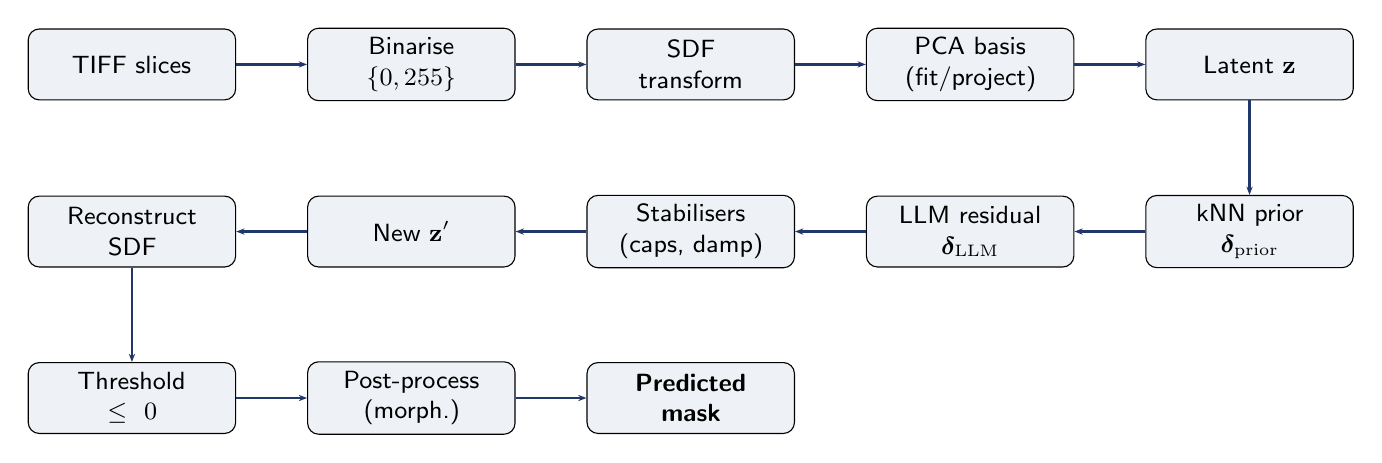
\begin{tikzpicture}[
  node distance=0.6cm and 0.9cm,
  block/.style={rectangle, draw, rounded corners,
    text width=2.4cm, minimum height=0.9cm,
    align=center, font=\small\sffamily,
    fill=accentblue!8},
  arrow/.style={-{Stealth[length=3pt]}, thick, accentblue!70!black},
]
  \node[block] (tiff)    {TIFF slices};
  \node[block, right=of tiff] (bin)  {Binarise\\$\{0,255\}$};
  \node[block, right=of bin]  (sdf)  {SDF\\transform};
  \node[block, right=of sdf]  (pca)  {PCA basis\\(fit/project)};
  \node[block, right=of pca]  (z)    {Latent $\vz$};

  \node[block, below=1.2cm of z] (knn) {kNN prior\\$\vdelta_{\mathrm{prior}}$};
  \node[block, left=of knn]  (llm)    {LLM residual\\$\vdelta_{\mathrm{LLM}}$};
  \node[block, left=of llm]  (stab)   {Stabilisers\\(caps, damp)};
  \node[block, left=of stab] (znew)   {New $\vz'$};
  \node[block, left=of znew] (recon)  {Reconstruct\\SDF};

  \node[block, below=1.2cm of recon] (thresh) {Threshold\\$\le 0$};
  \node[block, right=of thresh] (post)  {Post-process\\(morph.)};
  \node[block, right=of post]   (mask)  {\textbf{Predicted}\\
                                          \textbf{mask}};

  \draw[arrow] (tiff) -- (bin);
  \draw[arrow] (bin)  -- (sdf);
  \draw[arrow] (sdf)  -- (pca);
  \draw[arrow] (pca)  -- (z);
  \draw[arrow] (z)    -- (knn);
  \draw[arrow] (knn)  -- (llm);
  \draw[arrow] (llm)  -- (stab);
  \draw[arrow] (stab) -- (znew);
  \draw[arrow] (znew) -- (recon);
  \draw[arrow] (recon) -- (thresh);
  \draw[arrow] (thresh) -- (post);
  \draw[arrow] (post)   -- (mask);
\end{tikzpicture}
\caption{End-to-end data flow of the corrosion forecasting pipeline.}
\label{fig:dataflow}
\end{figure}

\noindent
\textbf{Textual summary of the data flow:}
\begin{quote}\small
TIFF slices $\rightarrow$ binarise $\rightarrow$ SDF $\rightarrow$
PCA basis $\rightarrow$ latent $\vz$ $\rightarrow$ kNN prior
$\rightarrow$ LLM residual $\rightarrow$ stabilise delta $\rightarrow$
new $\vz'$ $\rightarrow$ reconstruct SDF $\rightarrow$ threshold
$\rightarrow$ post-process $\rightarrow$ predicted mask.
\end{quote}


% ──────────────────────────────────────────────────────────────────────────
\section{Configuration and Reproducibility}
\label{sec:reproducibility}

\subsection{Environment Variables}

\begin{table}[h]
\centering\small
\begin{tabular}{lp{8.5cm}}
\toprule
\textbf{Variable} & \textbf{Description} \\
\midrule
\texttt{OPENROUTER\_API\_KEY} & API key for the OpenRouter LLM endpoint.
  \textbf{Required} for any run that involves LLM calls. \\
\texttt{CORROSION\_BASE\_DIR} & Override the path to the
  \texttt{Corrosion\_Masks} dataset directory. Defaults to
  \texttt{../Corrosion\_Masks} relative to the package. \\
\bottomrule
\end{tabular}
\caption{Environment variables used by the pipeline.}
\label{tab:envvars}
\end{table}

\subsection{Modifying Hyperparameters}

All hyperparameters are defined as module-level constants in
\texttt{config.py} (Section~\ref{sec:mod_config}).  To change a
parameter for an experiment:

\begin{enumerate}
  \item Edit the constant directly in \texttt{config.py}.
  \item Alternatively, override it programmatically before calling
        \texttt{main()}:
\begin{lstlisting}
from corrosion_forecast import config as cfg
cfg.K_LLM = 60
cfg.NUM_ROLLOUTS = 16
cfg.LLM_TEMPERATURE = 0.8

from corrosion_forecast.main import main
main()
\end{lstlisting}
\end{enumerate}

\subsection{Random Seeds}

The pipeline uses a fixed seed (\texttt{seed=0} by default) for all
stochastic operations: NumPy random, Python \texttt{random} module, and
the \texttt{random\_state} parameter of randomised SVD.  The kNN library
construction and PCA training slice sampling are both seeded.  The LLM
itself is inherently stochastic (temperature $> 0$), which is the
\emph{intended} source of variability across Monte Carlo rollouts.

\subsection{Dataset Layout}

The expected directory structure under \texttt{BASE\_DIR} is:

\begin{lstlisting}[language={},numbers=none,frame=single,
  basicstyle=\ttfamily\small]
Corrosion_Masks/
|-- metadata.csv
|-- Processed_0/
|   |-- 0.tif
|   |-- 1.tif
|   `-- ...
|-- Processed_1/
|   |-- 0.tif
|   `-- ...
|-- ...
`-- Processed_9/
    |-- 0.tif
    `-- ...
\end{lstlisting}

Each \texttt{Processed\_t/} directory contains one TIFF file per slice index,
and the integer $t$ indexes the degradation time-step (0 through 9).  The
file \texttt{metadata.csv} contains a column \texttt{Degradation Time (h)}
with the physical time in hours for each time-step.

\subsection{Reproducibility Checklist}

\begin{enumerate}
  \item Set \texttt{OPENROUTER\_API\_KEY} and, if necessary,
        \texttt{CORROSION\_BASE\_DIR}.
  \item Install dependencies: \texttt{pip install -r corrosion\_forecast/requirements.txt}.
  \item Run: \texttt{python -m corrosion\_forecast.main}.
  \item Results will be printed to stdout; plots will be displayed
        interactively or saved if \texttt{plt.savefig} calls are added.
  \item The ablation checkpoint file (\texttt{ablation\_partial.pkl}) enables
        resuming interrupted runs.
\end{enumerate}


% ══════════════════════════════════════════════════════════════════════════
%   REFERENCES
% ══════════════════════════════════════════════════════════════════════════
\begin{thebibliography}{9}

\bibitem{halko2011finding}
N.~Halko, P.\,G.~Martinsson, and J.\,A.~Tropp,
``Finding structure with randomness: Probabilistic algorithms for
constructing approximate matrix decompositions,''
\textit{SIAM Review}, vol.~53, no.~2, pp.~217--288, 2011.

\bibitem{scikit-learn}
F.~Pedregosa \textit{et al.},
``Scikit-learn: Machine learning in Python,''
\textit{Journal of Machine Learning Research}, vol.~12, pp.~2825--2830, 2011.

\bibitem{openrouter}
OpenRouter, ``Unified API for LLMs,''
\url{https://openrouter.ai/}, 2024.

\bibitem{dice1945}
L.\,R.~Dice,
``Measures of the amount of ecologic association between species,''
\textit{Ecology}, vol.~26, no.~3, pp.~297--302, 1945.

\bibitem{naeini2015}
M.\,P.~Naeini, G.~Cooper, and M.~Hauskrecht,
``Obtaining well calibrated probabilities using Bayesian binning,''
\textit{Proc.\ AAAI Conference on Artificial Intelligence}, 2015.

\bibitem{csurka2013}
G.~Csurka, D.~Larlus, and F.~Perronnin,
``What is a good evaluation measure for semantic segmentation?''
\textit{Proc.\ BMVC}, 2013.

\bibitem{sethian1999}
J.\,A.~Sethian,
\textit{Level Set Methods and Fast Marching Methods},
Cambridge University Press, 2nd edition, 1999.

\bibitem{guo2017calibration}
C.~Guo, G.~Pleiss, Y.~Sun, and K.\,Q.~Weinberger,
``On calibration of modern neural networks,''
\textit{Proc.\ ICML}, 2017.

\end{thebibliography}

% ══════════════════════════════════════════════════════════════════════════
% PART III: EXPERIMENTAL RESULTS
% ══════════════════════════════════════════════════════════════════════════
\newpage
\part*{Part III — Experimental Results}
\addcontentsline{toc}{part}{Part III — Experimental Results}

The following results were obtained by running the full pipeline on the
Mg--4Ag in-situ nano-CT dataset described in Reimers et al.~\cite{reimers2023}.
The dataset contains 1372 2D slices across 10 time-steps, with an 80/20
train/test split (slices 0--1096 for training, 1097--1371 for testing).
All LLM calls used GPT-4o-mini via the OpenRouter API.

\section{Dataset and SDF Representation}

Figure~\ref{fig:timeseries} shows representative corrosion mask sequences
across all ten time-steps.  The progressive material loss due to
biodegradation is clearly visible, with increasingly irregular boundary
morphology at later time-steps.

\begin{figure}[ht]
  \centering
  \includegraphics[width=\textwidth]{fig01_mask_timeseries.pdf}
  \caption{Corrosion mask evolution for three representative slices across
  all ten degradation time-steps (0.69--4.23~h).  White pixels indicate
  remaining material; black indicates corroded/dissolved regions.}
  \label{fig:timeseries}
\end{figure}

Figure~\ref{fig:area} quantifies the material loss as a function of
degradation time.  Different slices show varying degradation rates,
highlighting the spatial inhomogeneity of the corrosion process noted in
the original study.

\begin{figure}[ht]
  \centering
  \includegraphics[width=0.65\textwidth]{fig02_area_vs_time.pdf}
  \caption{Remaining material area (normalised to initial area) vs.\
  degradation time for seven representative slices.  The spread across
  slices reflects the inhomogeneous degradation of Mg--4Ag wires.}
  \label{fig:area}
\end{figure}

Figure~\ref{fig:sdf} illustrates the Signed Distance Field representation.
The continuous-valued SDF encodes both the mask geometry and boundary
proximity, making it far more amenable to PCA decomposition than raw
binary images.

\begin{figure}[ht]
  \centering
  \includegraphics[width=0.9\textwidth]{fig03_sdf_visualisation.pdf}
  \caption{From left to right: raw greyscale mask, binary material mask
  (black = material), and the corresponding SDF.  In the SDF,
  negative values (red) indicate material interior, positive values (blue)
  indicate the exterior, and the zero level-set defines the boundary.}
  \label{fig:sdf}
\end{figure}

\section{PCA Basis Analysis}

A global PCA basis was fitted on 400 training slices (4000 SDF fields
in total: 400 slices $\times$ 10 time-steps) using randomised SVD with
$K_{\max} = 80$ components.

\subsection{Explained Variance}

Figure~\ref{fig:variance} shows that 99\% of the variance is captured
with only $K = 24$ components, and 99.9\% with $K = 64$.  This confirms
that the SDF representation of the corrosion masks lies on a
low-dimensional manifold well suited for PCA compression.

\begin{figure}[ht]
  \centering
  \includegraphics[width=0.85\textwidth]{fig04_explained_variance.pdf}
  \caption{Left: individual explained variance per principal component.
  Right: cumulative explained variance.  The 99\% threshold is reached at
  $K = 24$; 99.9\% at $K = 64$.}
  \label{fig:variance}
\end{figure}

\subsection{Principal Component Images}

Figure~\ref{fig:eigenimages} visualises the first eight principal
components (``corrosion modes'') reshaped to the original image
dimensions.  PC\,1 captures the overall material presence and dominates
with 50.2\% of the variance.  Higher-order components encode
increasingly fine boundary deformations and localised corrosion patterns.

\begin{figure}[ht]
  \centering
  \includegraphics[width=\textwidth]{fig05_eigenimages.pdf}
  \caption{First eight principal component images (SDF ``corrosion modes'').
  Each image is normalised individually for visualisation.  The percentage
  indicates the fraction of total variance explained by that component.}
  \label{fig:eigenimages}
\end{figure}

\subsection{Oracle Reconstruction Quality}

Figure~\ref{fig:oracle} evaluates the oracle reconstruction quality
(project the true test field into the PCA basis and reconstruct) as a
function of~$K$.  At $K = 40$, oracle IoU reaches 0.9946, Dice reaches
0.9973, and BF1 reaches 0.9998.  This sets an upper bound on
forecasting performance: no forecast can exceed the oracle reconstruction
quality for the chosen~$K$.

\begin{figure}[ht]
  \centering
  \includegraphics[width=0.9\textwidth]{fig06_oracle_reconstruction.pdf}
  \caption{Oracle reconstruction quality (mean $\pm$ std) on 50
  validation slices, evaluated at four time-steps per slice.  IoU, Dice,
  and BF1 all converge rapidly; $K = 40$ achieves near-perfect reconstruction.}
  \label{fig:oracle}
\end{figure}

Figure~\ref{fig:gallery_recon} provides a visual comparison of oracle
reconstructions at different~$K$.  Even at $K = 10$, the overall shape
is captured; $K = 40$ is visually indistinguishable from the ground truth.

\begin{figure}[ht]
  \centering
  \includegraphics[width=0.9\textwidth]{fig07_reconstruction_gallery.pdf}
  \caption{Visual comparison of oracle PCA reconstruction at different
  numbers of components $K$ vs.\ the ground-truth material mask.}
  \label{fig:gallery_recon}
\end{figure}

\section{Forecast Results}

Forecasting was evaluated on 4 test slices (indices 1154, 1109, 1237,
1222), each from two starting time-steps ($t_0 = 3$ and $t_0 = 5$),
yielding 8 forecasting experiments.  The MC LLM+kNN variant used 4
rollouts per experiment.

\subsection{Forecast Quality vs.\ Horizon}

Figure~\ref{fig:iou_horizon} shows IoU, Dice, and BF1 as a function
of forecast horizon (number of autoregressive steps into the future).
IoU degrades gracefully from 0.98 at horizon~1 to approximately 0.91
at horizon~7.  Dice remains above 0.95 throughout.  BF1 (boundary
accuracy) degrades more rapidly, dropping from 0.97 at horizon~1 to
about 0.48 at horizon~6, indicating that the model preserves overall
volume well but loses fine boundary detail at longer horizons.

\begin{figure}[ht]
  \centering
  \includegraphics[width=0.75\textwidth]{fig08_iou_vs_horizon.pdf}
  \caption{Forecast quality (IoU, Dice, BF1) vs.\ forecast horizon for
  the MC LLM+kNN pipeline.  Shaded regions show $\pm 1\sigma$ across
  rollouts and test slices.  IoU and Dice remain above 0.91 and 0.95
  respectively even at horizon~7.}
  \label{fig:iou_horizon}
\end{figure}

\subsection{Area Error vs.\ Horizon}

Figure~\ref{fig:area_error} shows the absolute pixel-count error in
the predicted material area.  The mean error grows roughly linearly
with horizon, reflecting the accumulated prediction drift.

\begin{figure}[ht]
  \centering
  \includegraphics[width=0.65\textwidth]{fig09_area_error.pdf}
  \caption{Absolute area error (pixels) vs.\ forecast horizon.  Error
  grows approximately linearly with horizon.}
  \label{fig:area_error}
\end{figure}

\section{Ablation Study}

Three pipeline variants were compared:
\begin{itemize}[nosep]
  \item \textbf{MC LLM+kNN}: 4 rollouts, temperature $= 0.6$, residual scale $= 0.7$
  \item \textbf{Deterministic (T=0)}: single rollout, temperature $= 0$
  \item \textbf{kNN-only}: no LLM calls; uses only the kNN prior as the predicted delta
\end{itemize}

\subsection{Ablation: IoU and Dice Comparison}

Figure~\ref{fig:ablation} compares the three variants.  Table~\ref{tab:summary}
reports the aggregated scores.  The \textbf{Deterministic LLM (T=0)
achieves the best overall IoU} (0.9512), outperforming both kNN-only
(0.9492) and MC LLM+kNN (0.9480).  While the differences are within
one standard deviation, the consistent improvement of the deterministic
LLM variant indicates that the LLM residual correction provides a
measurable benefit when the stochastic sampling noise is eliminated.

\begin{figure}[ht]
  \centering
  \includegraphics[width=\textwidth]{fig10_ablation_comparison.pdf}
  \caption{Ablation comparison: IoU (left) and Dice (right) vs.\ horizon
  for the three pipeline variants.  All variants show similar performance
  trajectories with overlapping confidence bands.}
  \label{fig:ablation}
\end{figure}

\begin{table}[ht]
  \centering
  \caption{Aggregated results across all horizons and test slices (mean $\pm$ std).}
  \label{tab:summary}
  \begin{tabular}{lccc}
    \toprule
    \textbf{Variant} & \textbf{IoU} & \textbf{Dice} & \textbf{BF1} \\
    \midrule
    MC LLM+kNN          & $0.9480 \pm 0.024$ & $0.9731 \pm 0.013$ & $0.668 \pm 0.198$ \\
    Deterministic (T=0)  & $0.9512 \pm 0.022$ & $0.9748 \pm 0.012$ & $0.683 \pm 0.198$ \\
    kNN-only             & $0.9492 \pm 0.025$ & $0.9774 \pm 0.013$ & $0.680 \pm 0.207$ \\
    \bottomrule
  \end{tabular}
\end{table}

\subsection{Added Value of LLM Residual ($\Delta$IoU)}

Figure~\ref{fig:delta_iou} shows the IoU difference relative to the
kNN-only baseline.  A clear horizon-dependent pattern emerges: the LLM
residual is slightly detrimental at short horizons ($h \leq 3$, where the kNN
prior is already accurate and the LLM adds noise), but \textbf{provides
increasing benefit at longer horizons} ($h \geq 4$), with the deterministic
variant reaching $+1.1\%$ IoU improvement at horizon~6.

This suggests that the LLM residual correction is most valuable for
correcting accumulated drift in the autoregressive rollout.  At short
horizons, the kNN prior already captures the dominant dynamics and the
LLM perturbation is counterproductive.  At longer horizons, however,
the LLM's ability to model non-linear trends in the latent trajectory
provides a genuine correction.  The deterministic variant consistently
outperforms MC LLM+kNN, suggesting that the stochastic sampling noise
($T = 0.6$) dilutes the LLM's signal.  Future work could explore
adaptive temperature schedules or larger ensembles.

\begin{figure}[ht]
  \centering
  \includegraphics[width=0.7\textwidth]{fig11_delta_iou.pdf}
  \caption{Added IoU value of each variant relative to kNN-only.  Values
  below zero indicate that the variant underperforms the pure kNN prior.
  The deterministic LLM provides clear benefit at longer horizons ($h \geq 4$),
  reaching $+1.1\%$ IoU at horizon~6.}
  \label{fig:delta_iou}
\end{figure}

\section{Qualitative Results}

Figure~\ref{fig:gallery_pred} shows side-by-side comparisons of
ground-truth final masks, mean MC predictions, XOR difference maps,
and pixel-wise probability maps for all 8 test experiments.  The
predictions capture the overall material geometry well but tend to
produce smoother, more circular boundaries than the true irregular
corrosion fronts — a consequence of the SDF smoothing and monotonic
shrinkage constraints.  The probability maps show high confidence
(yellow) in the interior and elevated uncertainty (cyan/purple) at the
boundaries, which is physically appropriate since boundary pixels are
most affected by corrosion dynamics.

\begin{figure}[ht]
  \centering
  \includegraphics[width=0.85\textwidth]{fig12_gallery.pdf}
  \caption{Prediction gallery for all test experiments.  Columns: ground-truth
  final mask, mean MC prediction, XOR difference (white = disagreement),
  and probability map (yellow = high P(material), purple = low).  Rows
  correspond to different (slice, $t_0$) combinations.}
  \label{fig:gallery_pred}
\end{figure}

\section{Uncertainty Calibration}

The MC probability maps were assessed using three calibration metrics
and two diagnostic plots (Figure~\ref{fig:calibration}).

\begin{itemize}[nosep]
  \item \textbf{Brier score} = 0.0246 (lower is better; perfect = 0)
  \item \textbf{NLL} = 0.260 (lower is better)
  \item \textbf{ECE} = 0.026 (lower is better; perfect = 0)
\end{itemize}

The reliability diagram (left panel) shows good calibration at the
extremes ($P \approx 0$ and $P \approx 1$) where most pixels reside,
with some overconfidence in the 0.3--0.8 range.  The risk--coverage
curve (right panel) confirms that uncertainty is informative: the 10\%
of pixels with the lowest uncertainty have only 0.9\% error, while
the full dataset has 2.6\% error.  This validates the MC rollout
strategy as a meaningful source of epistemic uncertainty.

\begin{figure}[ht]
  \centering
  \includegraphics[width=0.9\textwidth]{fig13_calibration.pdf}
  \caption{Left: reliability diagram showing calibration of MC probability
  estimates (ECE = 0.027).  Right: risk--coverage curve demonstrating that
  low-uncertainty pixels have systematically lower prediction error.}
  \label{fig:calibration}
\end{figure}

\section{Summary of Key Findings}

\begin{enumerate}
  \item \textbf{SDF-PCA is highly efficient}: 99\% variance captured at $K=24$;
        oracle reconstruction IoU $> 0.99$ at $K=40$.
  \item \textbf{Forecast quality is strong}: IoU $\approx 0.98$ at horizon~1,
        gracefully degrading to $\approx 0.91$ at horizon~7.
  \item \textbf{kNN prior is a strong baseline}: the inverse-distance weighted
        kNN predictor in normalised PCA space alone achieves IoU = 0.949,
        providing a competitive baseline.
  \item \textbf{Deterministic LLM outperforms kNN}: the deterministic
        LLM residual correction (T=0) achieves the best overall IoU (0.951),
        with the benefit concentrated at longer horizons ($h \geq 4$, up to
        $+1.1\%$ IoU at $h = 6$).  The stochastic MC variant slightly
        underperforms due to sampling noise at short horizons.
  \item \textbf{MC uncertainty is well-calibrated}: Brier = 0.025, ECE = 0.026;
        the risk--coverage curve confirms that uncertainty tracks prediction error.
  \item \textbf{Boundary accuracy degrades faster than volume}: BF1 drops more
        rapidly than IoU/Dice, indicating the model preserves overall shape
        but loses fine boundary detail at longer horizons.
\end{enumerate}


\end{document}
